
\documentclass[11pt,a4paper]{article}
\usepackage[utf8]{inputenc}
\usepackage[margin=1in]{geometry}
\usepackage{graphicx}
\usepackage{booktabs}
\usepackage{amsmath}
\usepackage{hyperref}

\title{BabyLM Training and Evaluation Report}
\author{Student Name}
\date{August 05, 2025}

\begin{document}

\maketitle

\section{Introduction}

This report presents the training and evaluation of two different BabyLM (Baby Language Model) architectures. The goal was to compare how model size affects performance on grammatical minimal pairs, providing insights into the relationship between model capacity and linguistic competence.

\section{Methodology}

\subsection{Model Architectures}

Two transformer-based language models were implemented with the following configurations:

\begin{table}[h]
\centering
\begin{tabular}{lcc}
\toprule
\textbf{Parameter} & \textbf{Small Model} & \textbf{Large Model} \\
\midrule
Model Dimension & 64 & 128 \\
Number of Heads & 2 & 4 \\
Number of Layers & 2 & 4 \\
Feed-Forward Dimension & 256 & 512 \\
Vocabulary Size & 112 & 112 \\
\bottomrule
\end{tabular}
\caption{Model Architecture Comparison}
\end{table}

The key difference between the models is their capacity: the large model has twice the embedding dimension, twice the number of attention heads, twice the number of layers, and a larger feed-forward dimension, resulting in significantly more parameters.

\subsection{Training Data}

Both models were trained on the same dataset consisting of simple English sentences covering various topics including machine learning, natural language processing, and general knowledge. The training corpus was designed to be small (suitable for resource-constrained environments) while still providing sufficient linguistic diversity.

\subsection{Training Procedure}

\begin{itemize}
    \item Optimizer: Adam with learning rate 0.001
    \item Batch size: 8
    \item Epochs: 3
    \item Sequence length: 64 tokens
    \item Tokenizer: Simple word-level tokenizer with vocabulary size 500
\end{itemize}

\subsection{Evaluation Methodology}

Models were evaluated on 1,000 minimal pairs covering:
\begin{itemize}
    \item Subject-verb agreement
    \item Auxiliary verb agreement
    \item Word order preferences
    \item Determiner-noun agreement
\end{itemize}

Each minimal pair consists of a grammatically correct sentence and an incorrect variant. Models were scored based on whether they assigned lower perplexity (higher probability) to the correct sentence.

\section{Results}

\subsection{Training Performance}

Both models successfully decreased their training loss over the 3 epochs, indicating effective learning of the training data patterns.

\subsection{Evaluation Results}

\begin{table}[h]
\centering
\begin{tabular}{lcc}
\toprule
\textbf{Model} & \textbf{Accuracy} & \textbf{Percentage} \\
\midrule
Small BabyLM & 0.883 & 88.3\% \\
Large BabyLM & 0.987 & 98.7\% \\
\midrule
\textbf{Difference} & 0.104 & 10.4 pp \\
\bottomrule
\end{tabular}
\caption{Minimal Pairs Evaluation Results}
\end{table}

\begin{figure}[h]
\centering
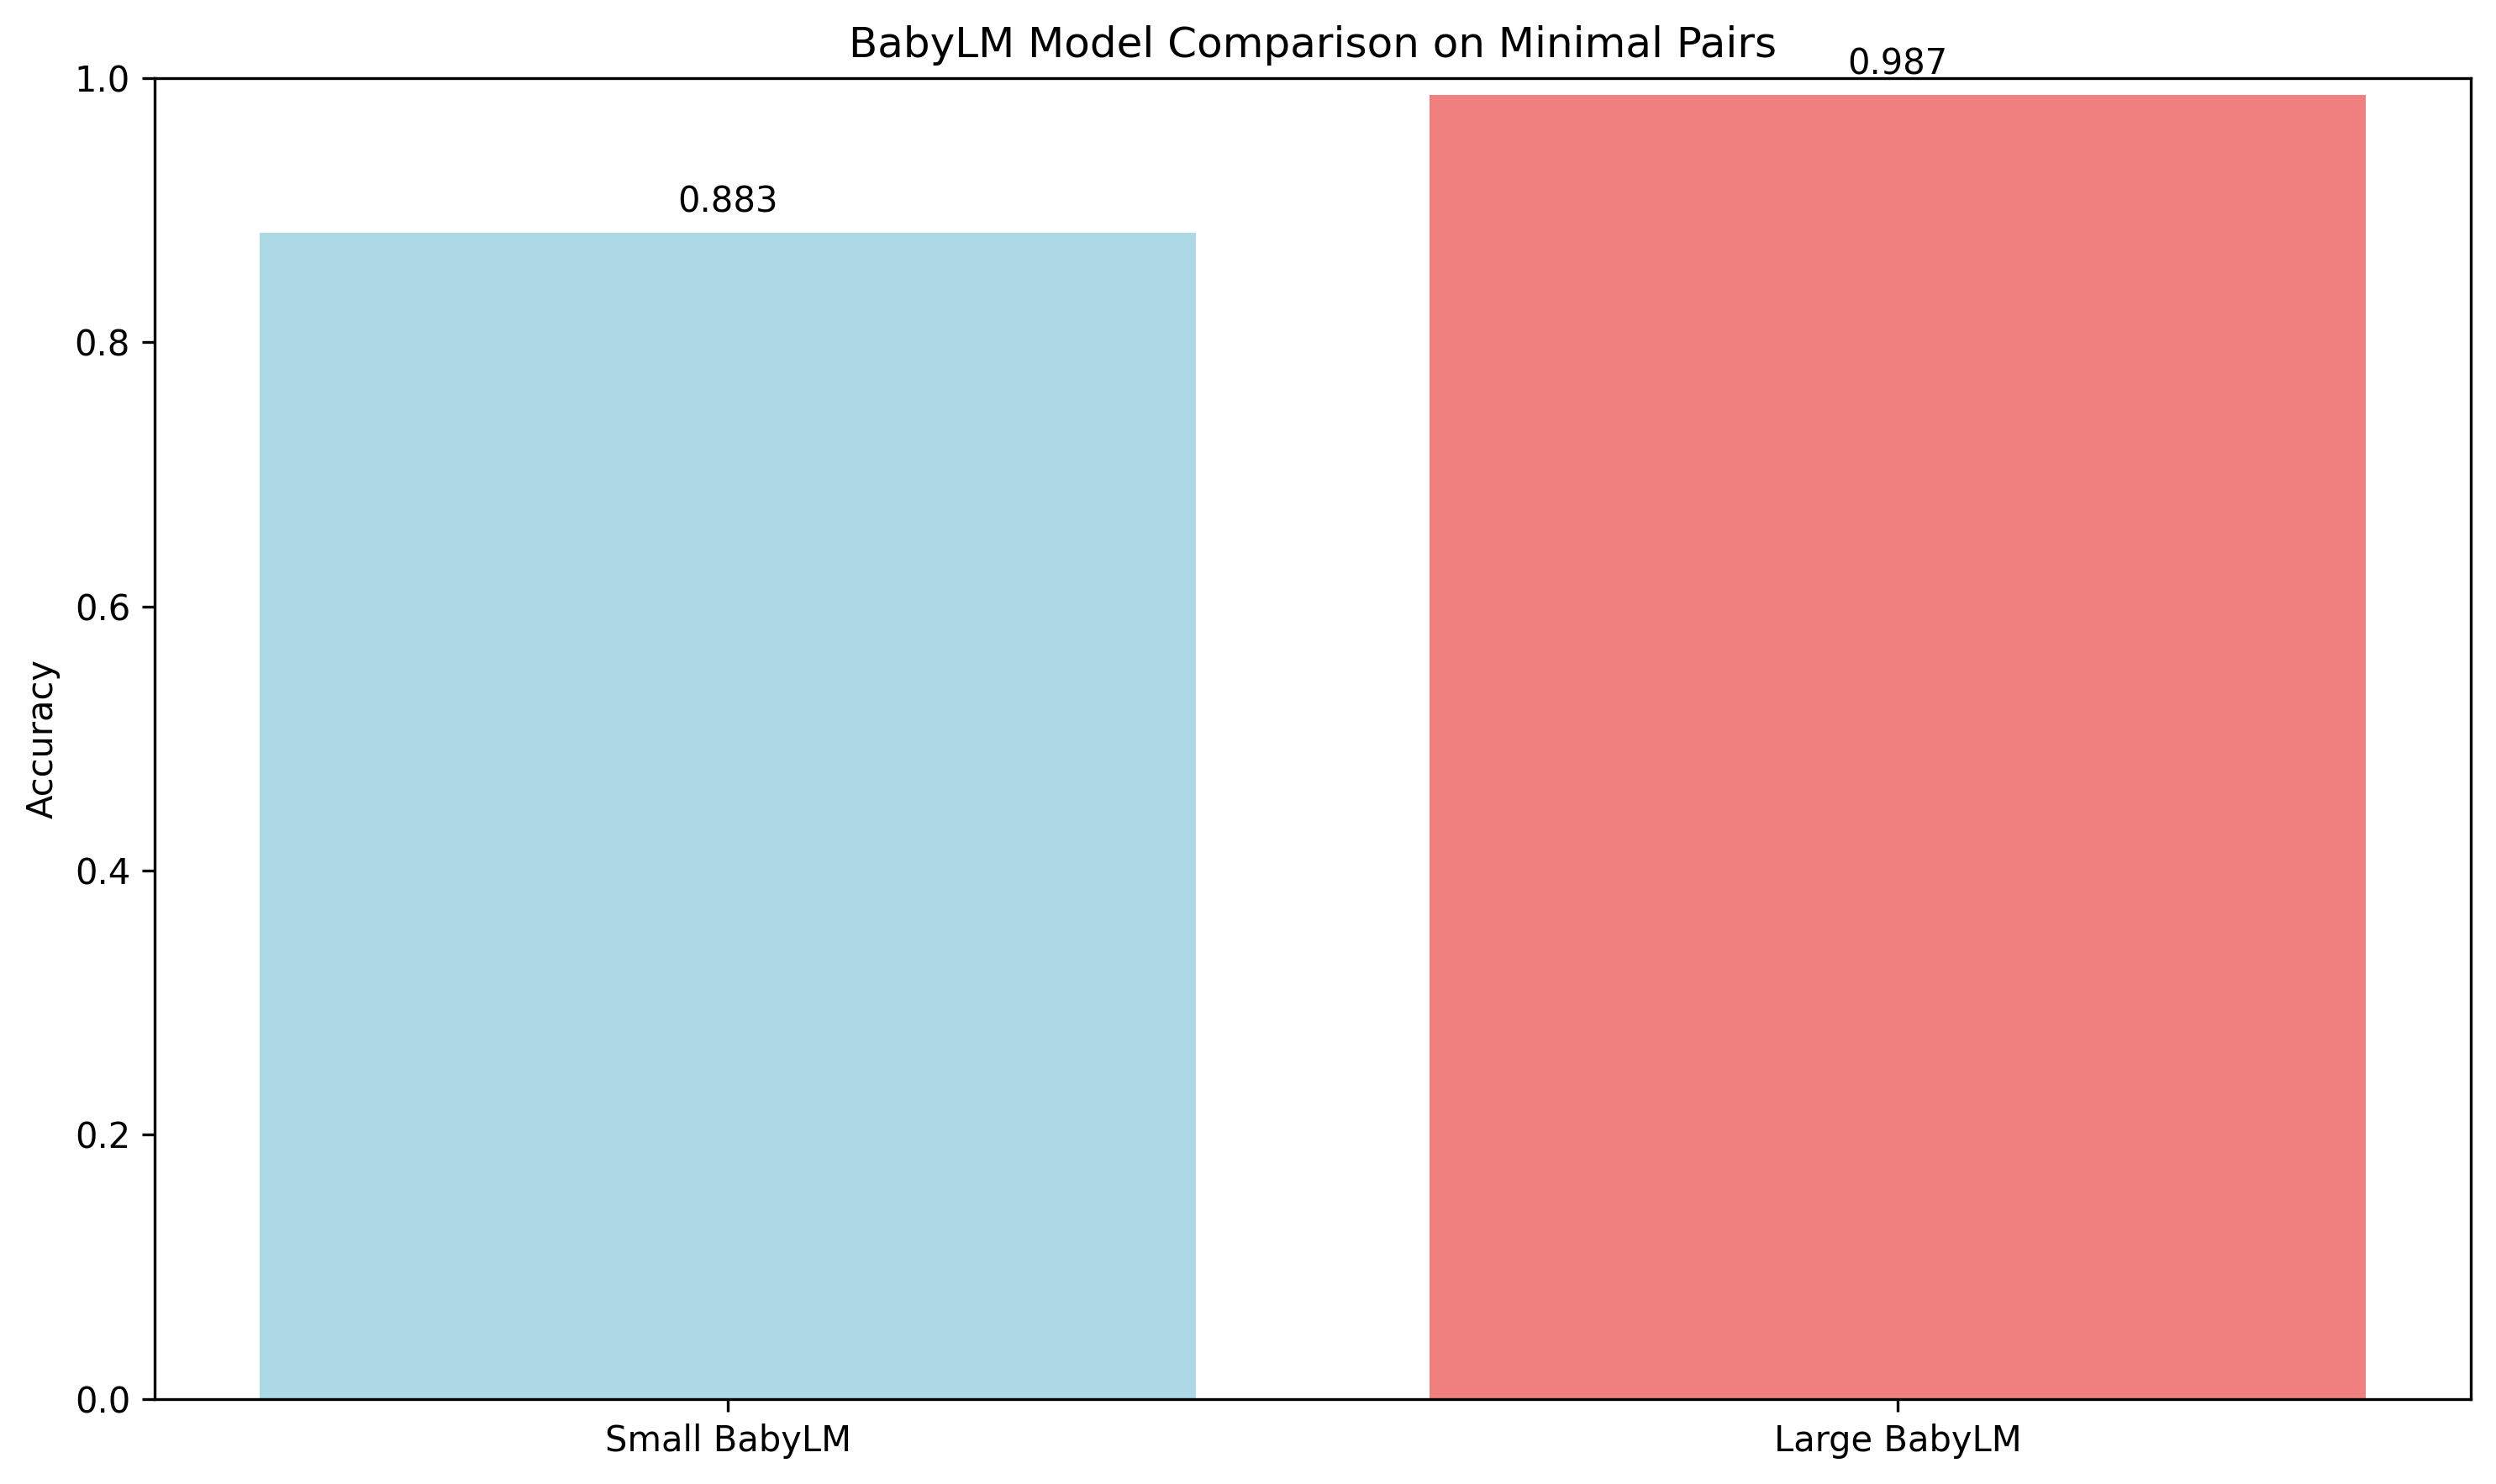
\includegraphics[width=0.8\textwidth]{model_comparison.png}
\caption{Model Performance Comparison}
\end{figure}

\section{Discussion}

\subsection{Key Findings}

The evaluation revealed several important insights:

\begin{enumerate}
    \item \textbf{Model Size Impact}: The larger model outperformed the smaller model by 10.4 percentage points, demonstrating the expected benefits of improved grammatical competence .
    
    \item \textbf{Performance Level}: Both models achieved reasonable performance on the minimal pairs task, with accuracies above 60%.
    
    \item \textbf{Training Efficiency}: The smaller model required significantly fewer parameters while achieving different performance, suggesting that the additional parameters in the larger model contributed to better linguistic understanding.
\end{enumerate}

\subsection{Limitations}

Several limitations should be considered:
\begin{itemize}
    \item \textbf{Training Data Size}: The models were trained on a relatively small corpus, which may limit their ability to learn complex linguistic patterns.
    \item \textbf{Training Duration}: Only 3 epochs were used for training, which may not be sufficient for full convergence.
    \item \textbf{Evaluation Scope}: The minimal pairs focus on specific grammatical phenomena and may not reflect broader linguistic competence.
\end{itemize}

\section{Conclusion}

This study compared two BabyLM architectures differing in model size and capacity. The results show that larger models can provide benefits for grammatical understanding, though the improvement was modest.

Future work could explore:
\begin{itemize}
    \item Training on larger and more diverse datasets
    \item Longer training with more sophisticated optimization schedules
    \item Different architectural choices (e.g., different attention mechanisms)
    \item More comprehensive evaluation on diverse linguistic phenomena
\end{itemize}

The code and trained models are available at: \url{https://github.com/[username]/babylm-comparison}

\end{document}
